\documentclass[border=10pt]{standalone}
\usepackage{tikz,amsmath}
\usetikzlibrary{arrows.meta,3d}

% ========== 颜色定义 ==========
\colorlet{myred}{red!80!black}
\colorlet{myblue}{blue!80!black}
\colorlet{mygreen}{green!60!black}

\begin{document}
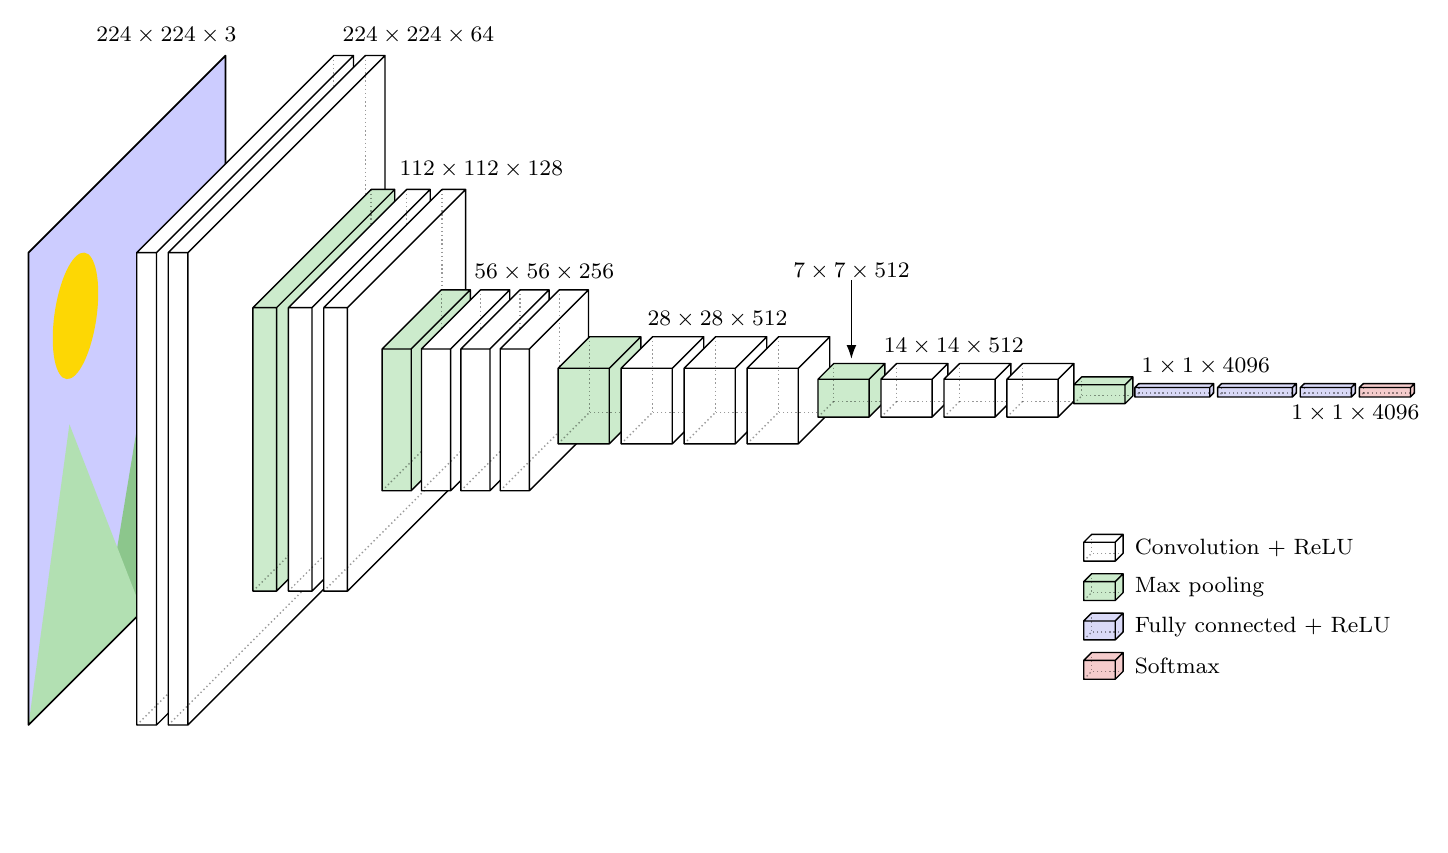
\begin{tikzpicture}[
    font=\footnotesize, scale=1, line join=round,
    every node/.style={outer sep=0pt, inner sep=0pt, align=center},
    w/.style={minimum width=#1},
    h/.style={minimum height=#1},
    s/.style={minimum size=#1},
    >={Latex[length=1.75mm, width=1.25mm]}
  ]

  % ========== 立方体绘制宏 ==========
  % #1,#2=位置  #3=侧边标签  #4,#5,#6=宽,高,深  #7=填充色
  \def\cube#1#2#3#4#5#6#7{%
    \begin{scope}[shift={(#1,#2)},scale=1]
      \pgfmathsetmacro{\cubex}{#4}
      \pgfmathsetmacro{\cubey}{#5}
      \pgfmathsetmacro{\cubez}{#6}
      \draw [draw=black, line width=.5pt,
             every edge/.append style={draw=black, opacity=.4, densely dotted},
             fill=#7, fill opacity=1]
        (\cubex/2,\cubey/2,\cubez/2) coordinate (o)
          -- ++(-\cubex,0,0) coordinate (a)
          -- ++(0,-\cubey,0) coordinate (b)
            edge coordinate [pos=1] (g) ++(0,0,-\cubez)
          -- ++(\cubex,0,0) coordinate (c) -- cycle
        (o) -- ++(0,0,-\cubez) coordinate (d)
          -- ++(0,-\cubey,0) coordinate (e) edge (g) -- (c) -- cycle
        (o) -- (a) -- ++(0,0,-\cubez) coordinate (f) edge (g) -- (d) -- cycle;
      \node[rotate=90, xshift=-2cm, yshift=.165cm] {#3};
    \end{scope}
  }

  % ========== 输入图像（TikZ 绘制，zy 平面）==========
  \begin{scope}[canvas is zy plane at x=0, transform shape]
    \fill[blue!20] (-3.25,-3) rectangle (3.25,3);                          % 天空
    \fill[yellow!75!orange] (1.7,1.6) circle (.75);                        % 太阳
    \fill[green!50!black!45] (-3.25,-3) -- (-1.1,.9) -- (.9,-3) -- cycle;  % 远山
    \fill[green!60!black!30] (-.5,-3) -- (1.9,.3) -- (3.25,-3) -- cycle;   % 近山
    \draw[black, line width=.6pt] (-3.25,-3) rectangle (3.25,3);           % 边框
  \end{scope}

  % ========== 立方体序列 ==========
  \cube{1.5}{0}{}{.25}{6}{6.5}{white}
  \cube{1.9}{0}{}{.25}{6}{6.5}{white}

  \cube{2.5}{0}{}{.3}{6*.6}{6.5*.6}{mygreen!20}
  \cube{2.95}{0}{}{.3}{6*.6}{6.5*.6}{white}
  \cube{3.4}{0}{}{.3}{6*.6}{6.5*.6}{white}

  \cube{3.8}{0}{}{.37}{6*.3}{6.5*.3}{mygreen!20}
  \cube{4.3}{0}{}{.37}{6*.3}{6.5*.3}{white}
  \cube{4.8}{0}{}{.37}{6*.3}{6.5*.3}{white}
  \cube{5.3}{0}{}{.37}{6*.3}{6.5*.3}{white}

  \cube{6}{0}{}{.65}{6*.16}{6.5*.16}{mygreen!20}
  \cube{6.8}{0}{}{.65}{6*.16}{6.5*.16}{white}
  \cube{7.6}{0}{}{.65}{6*.16}{6.5*.16}{white}
  \cube{8.4}{0}{}{.65}{6*.16}{6.5*.16}{white}

  \cube{9.2}{0}{}{.65}{6*.08}{6.5*.08}{mygreen!20}
  \cube{10}{0}{}{.65}{6*.08}{6.5*.08}{white}
  \cube{10.8}{0}{}{.65}{6*.08}{6.5*.08}{white}
  \cube{11.6}{0}{}{.65}{6*.08}{6.5*.08}{white}

  \cube{12.4}{0}{}{.65}{6*.04}{6.5*.04}{mygreen!20}

  \cube{13.3}{0}{}{.95}{6*.02}{6.5*.02}{myblue!15}
  \cube{14.35}{0}{}{.95}{6*.02}{6.5*.02}{myblue!15}
  \cube{15.25}{0}{}{.65}{6*.02}{6.5*.02}{myblue!15}

  \cube{16}{0}{}{.65}{6*.02}{6.5*.02}{myred!20}

  % ========== 图例 ==========
  \cube{12.4}{-2}{}{.4}{6*.04}{6.5*.04}{white}
  \cube{12.4}{-2.5}{}{.4}{6*.04}{6.5*.04}{mygreen!20}
  \cube{12.4}{-3}{}{.4}{6*.04}{6.5*.04}{myblue!15}
  \cube{12.4}{-3.5}{}{.4}{6*.04}{6.5*.04}{myred!20}

  \node[anchor=west] at (12.8,-2) {Convolution $+$ ReLU};
  \node[anchor=west] at (12.8,-2.5) {Max pooling};
  \node[anchor=west] at (12.8,-3) {Fully connected $+$ ReLU};
  \node[anchor=west] at (12.8,-3.5) {Softmax};

  % ========== 尺寸标注 ==========
  \node at (0.5,4.5) {$224 \times 224 \times 3$};
  \node at (3.7,4.5) {$224 \times 224 \times 64$};
  \node at (4.5,2.8) {$112 \times 112 \times 128$};
  \node at (5.3,1.5) {$56 \times 56 \times 256$};
  \node at (7.5,.9) {$28 \times 28 \times 512$};
  \node at (10.5,.55) {$14 \times 14 \times 512$};
  \node at (13.7,.3) {$1 \times 1 \times 4096$};
  \node at (15.6,-.3) {$1 \times 1 \times 4096$};

  \draw[<-] (9.2,.4) -- node[pos=1,above] {$7 \times 7 \times 512$} +(0,1);

\end{tikzpicture}
\end{document}